\begin{samplecase}
{\bf Inelastic spectra at 20 MeV: Direct + Preeq + GR + Compound}\newline
For pre-equilibrium studies, it may be worthwhile to distinguish between the 
various components of the emission spectrum. This was already mentioned in 
sample case (1c). As an extra sample case, we compare the calculated 
${}^{209}$Bi(n,xn) spectrum at 20 MeV with experimental data. This is 
accomplished with the following input file,

\VerbatimInput{\samples n-Bi209-spec/org/talys.inp}

The various components of the spectrum, and the total, as present in the file
{\em nspec020.000.tot}, are plotted in Fig.~\ref{bi209nspec}.
\end{samplecase}
\begin{figure}
\centering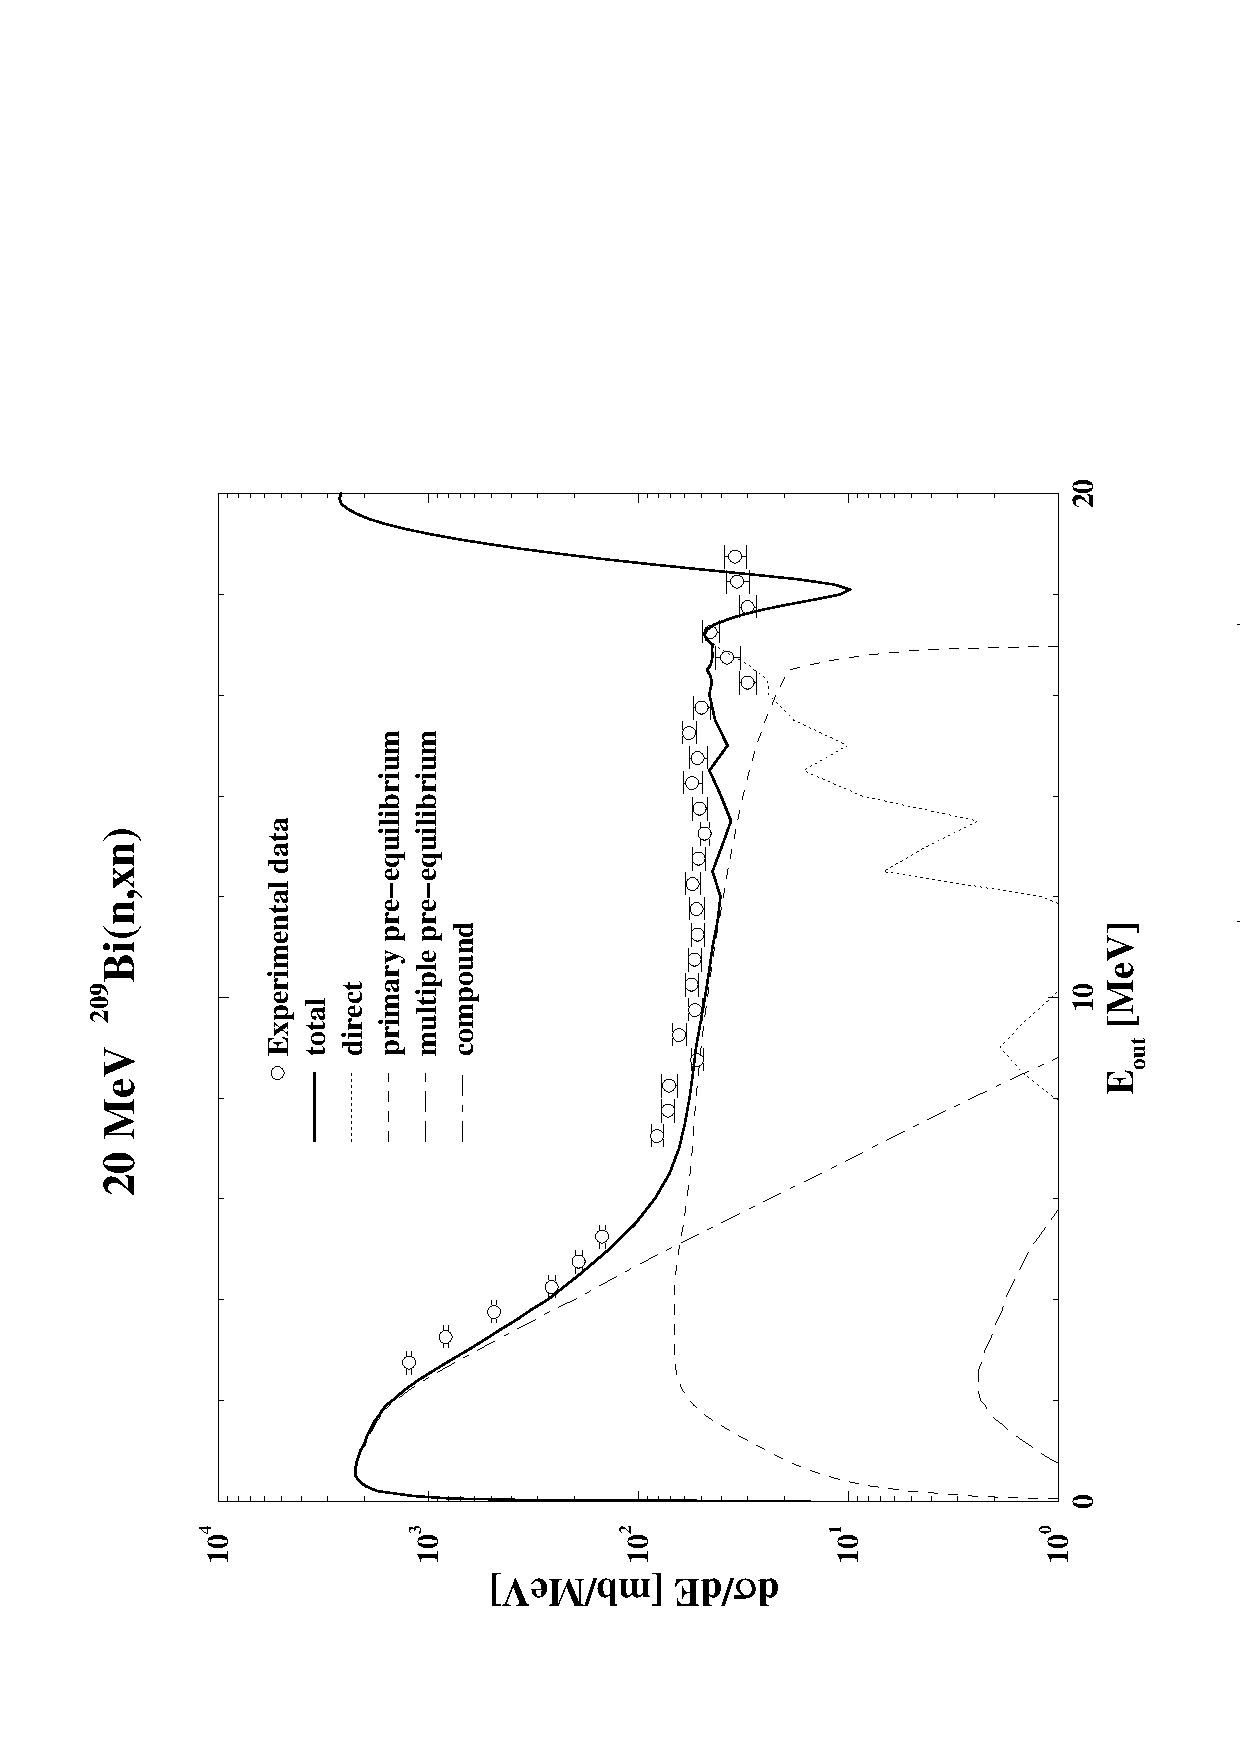
\includegraphics[scale=0.6,angle=270]{bi209nspec}
\caption{${}^{209}$Bi (n,xn) spectrum at 20 MeV. Experimental data are
obtained from \protect\cite{Marcinkowski1991}.}
\label{bi209nspec}
\end{figure}
